% !TEX program = xelatex
% \documentclass[usenames,xcolor=svgnames,11pt,sans,handout]{beamer}
\documentclass[usenames,xcolor=svgnames,11pt,sans]{beamer}
\usetheme{Madrid}
\colorlet{theme}{DarkGreen}
\usecolortheme[named=theme]{structure}
\newcommand{\key}[1]{{\color{theme} #1}}

\usepackage{xeCJK}
\setCJKmainfont{SimHei}
\usepackage[T1]{fontenc}
\usepackage{zi4}

\usepackage{siunitx}

\usepackage{listings}
\lstset{
    language=[LaTeX]TeX,
    xleftmargin=2em,
    keywordstyle=\color{theme},
    basicstyle=\ttfamily,
    basewidth={.5em,.5em},
    escapeinside={<@}{@>}
}

\usepackage{tikz}
\usetikzlibrary{positioning, arrows, shapes, shapes.multipart, backgrounds, calc, automata}
\usepackage{tikz-cd} % for demo/cd.tex
\usepackage{forest} % for demo/ast.tex

\let\t\texttt
\newcommand{\optional}{$^{\color{theme} ?}$}

\begin{document}

% credits
\title{Ti$k$Z 画“图”指南}
\subtitle{(从用户的角度出发)}
\author{Paul}
\date{2020-10-31}

% contents
\AtBeginSection[]
{
    \begin{frame}{目录}
        \tableofcontents[currentsection]
    \end{frame}
}

\AtBeginSubsection[]
{
    \begin{frame}{目录}
        \tableofcontents[currentsubsection]
	\end{frame}
}

% titlepage
\begin{frame}
    \titlepage
\end{frame}

\begin{frame}
    \begin{center}\Large
        这是一个\key{技术}和\key{非技术}报告
    \end{center}
\end{frame}

\section{Ti$k$Z 是啥}

\begin{frame}
    \frametitle{口号}

    \begin{quote}\Large
        Ti$k$Z ist kein Zeichenprogramm.

        \rightline{-- by Till Tantau}
    \end{quote}
\end{frame}

\begin{frame}
    \frametitle{Ti$k$Z 能干啥}

    \begin{itemize}
        \item 画(计算机科学里的)树
        \item 画(计算机科学里的)图
        \item 画统计图、曲线图
        \item 画三维图形
        \item 画思维导图
        \item ……
    \end{itemize}

    \pause
    \vspace{20pt}
    \begin{center}\Large\color{theme}
        “Ti$k$Z 画不出来的图,就是不需要画的图”
    \end{center}
\end{frame}

\begin{frame}
    \frametitle{常见问题}

    \begin{itemize}
        \item 我用 \LaTeX 排版,是不是所有图都要用 Ti$k$Z 画?
        \pause
        \item Ti$k$Z 和专业作图软件 MS Word/Powerpoint 等相比,谁更好用?
        \pause
        \item Ti$k$Z 和专业统计软件 MS Excel, Python 等相比,谁更好用?
    \end{itemize}

    \pause
    \vspace{20pt}
    It's up to you: \t{ppt.tex}, or \t{beamer.pptx}, or whatever!
\end{frame}

\section{例子,例子}

\begin{frame}
    \frametitle{Total Store Order}

    \centering\tikzstyle{executed} = [circle, draw=black, fill=gray]

\begin{tikzpicture}
    \node (i1) {ST};
    \node [below=of i1] (i2) {LD};
    \node [right=of i2] (x1) {};
    \node [right=of x1] (x) {Memory};
    \node [executed, below=of x] (d2) {};
    \node [executed, below=of d2] (d1) {};
    \node [below=of d1] (y) {};

    \draw [->] (i1) -- (d1);
    \draw [->] (i2) -- (d2);
    \draw [dashed,-] (x) -- (y);
\end{tikzpicture}
\end{frame}

\begin{frame}[fragile]
    \frametitle{基本语法}

    \begin{lstlisting}
\node [选项]<@\optional@> (名称)<@\optional@> {文本};

\draw [选项]<@\optional@> (起点名称) 连接方式 (终点名称);
    \end{lstlisting}
\end{frame}

\begin{frame}
    \frametitle{Markov Chain}

    \centering\usetikzlibrary{automata}
\tikzstyle{mcstate} = [state, fill=gray!20!white]

\begin{tikzpicture}[draw=Green, very thick, >=latex', auto]
    \node [mcstate]                 (s4) {4};
    \node [mcstate, right=of s4]    (s1) {1};
    \node [mcstate, below=of s4]    (s2) {2};
    \node [mcstate, right=of s2]    (s6) {6};
    \node [mcstate, right=of s1]    (s5) {5};
    \node [mcstate, above=of s1]    (s3) {3};
    
    \draw [->]
        (s4) edge [loop left] node {1/3} (s4)
        (s4) edge [above]     node {1/3} (s1)
        (s4) edge             node {1/3} (s2)
        (s1) edge             node {1} (s3)
        (s3) edge [above]     node {1} (s5)
        (s5) edge             node {1} (s1)
        (s2) edge [bend left] node {1} (s6)
        (s6) edge [bend left] node {1/2} (s2)
        (s6) edge [loop right] node {1/2} (s6)
    ;
\end{tikzpicture}
\end{frame}

\begin{frame}
    \frametitle{Petri Net}

    \centering\usetikzlibrary{petri}
\tikzstyle{red place} = [place, draw=red!75, fill=red!20]
\tikzstyle{red transition} = [transition, thick, draw=red!75, fill=red!20]

\begin{tikzpicture}[auto, node distance=3em, >=stealth', bend angle=30]
    \node [place, tokens=1, label=$p_1$] (p1) 				{};
    \node [transition, label=$t_1$] 	 (t1) [right=of p1] {};
    \node [place, label=$p_2$] 			 (p2) [right=of t1] {};
    \node [transition, label=right:$t_2$] 	 (t2) [right=of p2] {};
    \node [red place, label=$p_3$]	 (p3) [above=of t2] {};
    \node [red place, tokens=2, label=below:$p_4$] (p4) [below=of t2] {};
    \node [red transition, label=$t_4$] 	 (t4) [right=of t2] {};
    \node [red place, tokens=1, label=$p_5$] (p5) [right=of t4] {};
    \node [transition, label=$t_3$]      (t3) [right=of p4] {};

    \draw [->]
        (p1) edge (t1)
        (t1) edge [bend left] (p3)
        (t1) edge (p2)
        (t1) edge [bend left=5] (p4)
        (t1) edge [bend right=5] (p4)
        (p2) edge [bend right] (t2)
        (t2) edge [bend right] (p2)
        (p3) edge (t2)
        (p4) edge (t2)
        (p4) edge [bend left=10] (t3)
        (p4) edge [bend right=10] (t3)
        (t3) edge (p5)
    ;

    \draw [->, draw=red!75, fill=red!75]
        (t4) edge [bend left] (p3)
        (t4) edge [bend right] (p4)
        (p5) edge (t4)
    ;
\end{tikzpicture}
\end{frame}

\begin{frame}
    \frametitle{Process}

    \centering\tikzstyle{io} = [rectangle, text centered, text width=7em, fill=green!20]
\tikzstyle{proc} = [rectangle, fill=blue!20, text width=7em, text centered, rounded corners]
\tikzstyle{decision} = [diamond, fill=blue!20, text centered, aspect=2]
\tikzstyle{entity} = [text centered, text width=8em, fill=red!20]
\tikzstyle{line} = [draw, -latex']

\begin{tikzpicture}[auto, every text node part/.style={align=center}, every path/.style={->}]
    \node [io] (grammar) {(refined) grammar};
    \node [decision, below=of grammar] (ambig) {ambiguous?};
    \node [below right=.5 and .5 of ambig] (stop) {done};
    \node [proc, below=of ambig] (gen) {ambiguous word generator};
    \node [proc, right=of ambig] (synt) {grammar refinement};
    \node [entity, right=4.3 of gen] (select) {user interaction};
    \node [entity, right=4.3 of grammar] (input) {initial grammar};
    \node [below=.25 of select, red] {user};

    \path [line, red, thick] (input) -- node [above] {input} (grammar);
    \path [line] (grammar) -- (ambig);
    \path [line] (ambig.east) -| node {no} (stop);
    \path [line] (ambig) -- node {yes} (gen);
    \path [line] (gen) -- node [below] {ambiguous word \& \\ parse trees} (select);
    \path [line, red, thick] (select) -- node [right, pos=0.6] {feedback} (synt);
    \path [line] (synt) -- node [right, pos=0.7] {add restrictions} (grammar);
    % Draw user rectangle
    \draw [red, thick, dashed, rounded corners]
        ($(select.south east)+(.25,-.25)$) rectangle ($(input.north west)+(-.25,.25)$);
\end{tikzpicture}

\end{frame}

\begin{frame}
    \frametitle{常用选项}

    \begin{itemize}
        \item 边框:\t{draw},填充:\t{fill}
        \item 颜色、粗细、线型:使用“形容词”
        \item 位置:\t{below}, \t{above}, \t{left}, \t{right}
        \item 结点标签:\t{label}
        \item 自动控制箭头标注的位置:\t{auto}
        \item 箭头类型:\t{<start tip>-<end tip>}
    \end{itemize}
\end{frame}

\begin{frame}
    \frametitle{长度单位}

    除了普通人都知道的(如 \si{cm})以外,还可能用到:
    \begin{itemize}
        \item \si{pt} (\SI{1}{pt} = \SI{0.351}{mm})
        \item \si{in} (\SI{1}{in} = \SI{25.4}{mm})
        \item \si{em}(当前字体中 M 的宽度)
        \item \si{ex}(当前字体中 x 的高度)
    \end{itemize}
\end{frame}

\begin{frame}
    \frametitle{Strongly Connected Component}

    \centering\tikzstyle{scc node} = [state, fill=gray!20!white]

\begin{tikzpicture}[every loop, auto=left, very thick, >=latex', draw=Blue, fill=Blue]
    \begin{scope}[local bounding box=scc]
        \node [scc node, initial]        (s0) {$s_0$};
        \node [scc node, right=of s0]    (s1) {$s_1$};
        \draw
            (s0) edge [bend left] node {0.5} (s1)
            (s1) edge [bend left] node {0.5} (s0)
        ;
        \begin{pgfonlayer}{background}
            \path[fill=blue!20,draw=blue,dashed,thick,rounded corners]
                (scc.south west) rectangle
                ($(scc.north east) + (0.2cm,0cm)$);
        \end{pgfonlayer}
    \end{scope}

    \begin{scope}[local bounding box=bscc1]
        \node[scc node, right=2.5cm of s1, label=right:$\{d\}$]    (s2) {$s_2$};
        \node[scc node, below=of s2, label=right:$\{c\}$]    (s5) {$s_5$};
        \draw
            (s2) edge [bend left] node {1} (s5)
            (s5) edge [bend left] node {1} (s2)
            ;
        \begin{pgfonlayer}{background}
            \path[fill=red!20,draw=red,dashed,thick,rounded corners]
                ($(bscc1.south west) - (0cm,0.2cm)$) rectangle
                ($(bscc1.north east) + (0cm,0.2cm)$);
        \end{pgfonlayer}
    \end{scope}

    \begin{scope}[local bounding box=bscc2]
        \node[scc node, below=1.3cm of s0, label=left:$\{b\}$]    (s3) {$s_3$};
        \draw (s3) edge [loop below] node {1} (s3);
        \begin{pgfonlayer}{background}
            \path[fill=red!20,draw=red,dashed,thick,rounded corners]
                (bscc2.south west) rectangle
                ($(bscc2.north east) + (0.2cm,0.2cm)$);
        \end{pgfonlayer}
    \end{scope}

    \begin{scope}[local bounding box=bscc3]
        \node[scc node, below=1.3cm of s1, label=right:$\{b\}$]    (s4) {$s_4$};
        \draw (s4) edge [loop below] node {1} (s4);
        \begin{pgfonlayer}{background}
            \path[fill=red!20,draw=red,dashed,thick,rounded corners]
                ($(bscc3.south west) - (0.2cm,0cm)$) rectangle
                ($(bscc3.north east) + (0cm,0.2cm)$);
        \end{pgfonlayer}
    \end{scope}

    \draw
        (s1) edge node {0.25} (s2)
        (s1) edge node {0.25} (s4)
        (s0) edge node {0.5} (s3)
    ;
\end{tikzpicture}
\end{frame}

\begin{frame}
    \frametitle{Commutative Diagram\footnote{\url{https://tex.stackexchange.com/questions/468894/diagrams-in-category-theory}}}

    \centering% https://tex.stackexchange.com/questions/468894/diagrams-in-category-theory

\begin{tikzcd}[sep=4em]
      A \arrow[r, "b"] \arrow[d, "g"] 
    & C \arrow[r, "\alpha"] \arrow[d, "\gamma", pos=0.4, swap]
    & D \arrow[d, "\beta"] \\
      B \arrow[rru, "h", pos=0.7, swap]
    & B' \arrow[r, "\omega"]
    & D'
\end{tikzcd}
\end{frame}

\begin{frame}
    \frametitle{Parse Tree}

    \begin{center}
        \footnotesize\begin{forest}
    for tree={align=center}
    [\t{MethodDef}
        [...]
        [\t{Type}
            [{\t{VOID} \\ ``\t{void}''}]
        ]
        [...]
        [\t{MethodBody}
            [\t{StmtList}
                [\t{Stmt}
                    [\t{LocalVarDecl}
                        [\t{Type}
                            [\t{BaseType}
                                [{\t{FLOAT}\\``\t{float}''}]
                            ]
                        ]
                        [\t{VarDecl}
                            [{\t{ID}\\``\t{SommeCar}''}]
                            [...]
                        ]
                    ]
                ]
                [\t{Stmt}
                    [\t{ReturnStmt}, tikz={
                        \node [draw=red, rounded corners, fit to=tree,inner sep=0] {};
                     }
                        [{\t{RETURN}\\``\t{return}''}]
                        [{\t{ID}\\``\t{SommeCar}''}]
                    ]
                ]
            ]
        ]
    ]
\end{forest}

    \end{center}
\end{frame}

\begin{frame}
    \frametitle{调库}

    \begin{itemize}
        \item 常用:\t{positioning, arrows, shapes}
        \item 坐标计算:\t{calc}
        \item 领域特定:\t{automata}, \t{petri}, \t{circuit}, \t{matrix}
        \item 扩展性的宏包:\t{forest}, \t{tikz-cd}
    \end{itemize}
\end{frame}

\begin{frame}
    \frametitle{Matrix\footnote{从官方文档中截取的例子}}

    \centering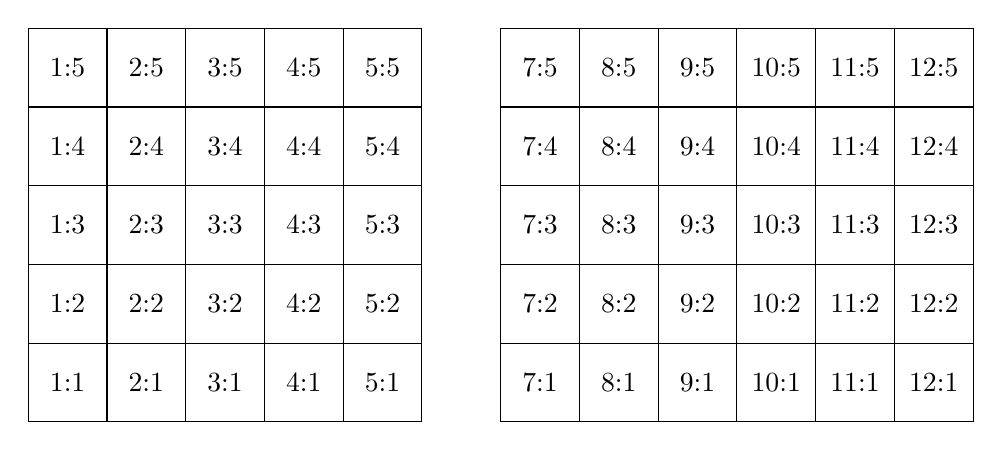
\begin{tikzpicture}
    \foreach \x in {1,2,...,5,7,8,...,12} {
        \foreach \y in {1,...,5} {
            \draw (\x,\y) +(-.5,-.5) rectangle ++(.5,.5);
            \draw (\x,\y) node {\x:\y};
        }
    }
\end{tikzpicture}
\end{frame}

\begin{frame}[fragile]
    \frametitle{Mutual References}

    \lstinputlisting{demo/mutual.tex}

    \begin{center}
        % \tikzstyle{my node1} = [state, thick, my node2]
\tikzstyle{my node2} = [my node1, orange]

\begin{tikzpicture}
    \node [my node1] (x) {$x$};
    \node [my node2, right=of x] {$y$};
\end{tikzpicture}        
    \end{center}
\end{frame}

\section{总结}

\begin{frame}
    \frametitle{学习资料}

    \begin{itemize}
        \item \t{texdoc tikz}
        \item \url{https://texample.net/tikz/examples/}
    \end{itemize}
\end{frame}

\begin{frame}
    \frametitle{Ti$k$Z 使用技巧}

    \begin{itemize}
        \item 写代码前手画草图
        \pause
        \item 错误信息有时候有用,没用的时候看看是不是语法错了
        \pause
        \item 方向不对,多试几次
    \end{itemize}
\end{frame}

\begin{frame}
    \frametitle{Repo}

    \centering\Large
    
    \url{https://github.com/paulzfm/TikZ-Tunight}

    \vspace{10pt}
    Check the \key{main} branch!
\end{frame}

\end{document}